% Chapter 5

\chapter{Results}
\label{chap:results}

\section{Turbulence-specific Post-processing}

In order to make available, all of the turbulence-specific post-processing from a given simulation output of \texttt{PySPH} \parencite{ramachandran2021a}, generated through the \texttt{Application} class, a \texttt{TurbulentFlowApp} class was created. This class inherits from the \texttt{Application} class and adds additional post-processing attributes and methods, such as:

\begin{itemize}
	\item class attributes:
	\begin{itemize}
		\item number of interpolation points along each axis,
		\item kernel to be used for the interpolation, and the corresponding kernel radius,
		\item interpolation method,
		\item norm order to be used for the computation of the $1D$ energy spectrum (\textit{also referred to as the scalar energy spectrum}),
		\item expected slope for the $1D$ energy spectrum,
        \item type of FTLE field (either \textit{forward} or \textit{backward}),
	\end{itemize}
	
	\item class methods:
	\begin{itemize}
		\item \texttt{compute\_interpolated\_vel\_field}: to compute the interpolated velocity field, at specified indices of the output files,
        \item \texttt{compute\_ek}: to compute the $1D$ energy spectrum from the corresponding interpolated velocity field,
        \item \texttt{compute\_ek\_slope}: to compute the slope of the $1D$ energy spectrum, using the \texttt{scipy.stats.linregress} function,
        \item \texttt{compute\_ftle}: to compute the FTLE (Finite-time Lyapunov Exponent) field, using the corresponding interpolated velocity field between two specific output files,
        \item plotter functions, that can either plot the $1D$ energy spectrum for a specific output file (along with a fit line), or plot the evolution of the $1D$ energy spectrum over a range of output files, or plot the FTLE field.
	\end{itemize}
\end{itemize}

The derived class is also coded to log the details of the interpolator used, which includes details on the kernel, radius scale, problem dimension, SPH equations involved in the interpolation scheme in the original \texttt{problem.log} file created by the default \texttt{Application} class. This enables the user to keep track all of the relevant details of the simulation including its post-processing, in a single log file.

The following subsections, detail the implementation of the energy spectrum and FTLE field computation, and important observations made from the same.


\subsection{Energy Spectral Density}
In order to compute the energy spectrum, the following steps are performed:

\begin{itemize}
    \item the velocity field is interpolated along a grid of uniformly spaced rectangular points,
    \item the velocity field is then transformed to Fourier space, using the \texttt{numpy.fft.fftn} function, and subsequently normalized as given as
    \begin{equation}
        \hat{\vect{v_i}}(\vect{k}) = \frac{ fft\{ \vect{v_i}(\vect{r}) \} }{U_0 \times len(\vect{v_i})}
    \end{equation}
    where $U_0$ is a reference velocity and $\vect{v_i}$ is the $i^{th}$ component of the velocity field,
    \item the corresponding energy spectrum is then computed as
    \begin{equation}
        \vect{E_i}(\vect{k}) = \frac{1}{2} \hat{\vect{v_i}}^2
    \end{equation}
    \item the $1D$ energy spectrum $E(k)$ is then computed from the energy vector field $\vect{E_i}(k_x, k_y, k_z)$, by integrating it over the surface of a sphere of appropriate dimension between the limits $k=0$ and $k=k_{max}$, where $k_{max}$ is the maximum wavenumber of the energy spectrum, where 
    \begin{equation}
        k_{max} = round(1 + ceil(|(l_x, l_y, l_z)|/2))
    \end{equation}
\end{itemize}

The function to compute the $1D$ energy spectrum was coded using three different backends, namely, pure \texttt{python}, \texttt{numba} \parencite{Lam_Pitrou_Seibert_2015}, and \texttt{compyle} \parencite{compyle_pr_ab-proc-scipy-2020}.
The speedup results of the three-implementations are shown in \figref{fig:espec-dim-1}, \figref{fig:espec-dim-2}, and \figref{fig:espec-dim-3} for $1D$, $2D$, and $3D$ velocity fields respectively.

\begin{figure}[h]
	\centering
	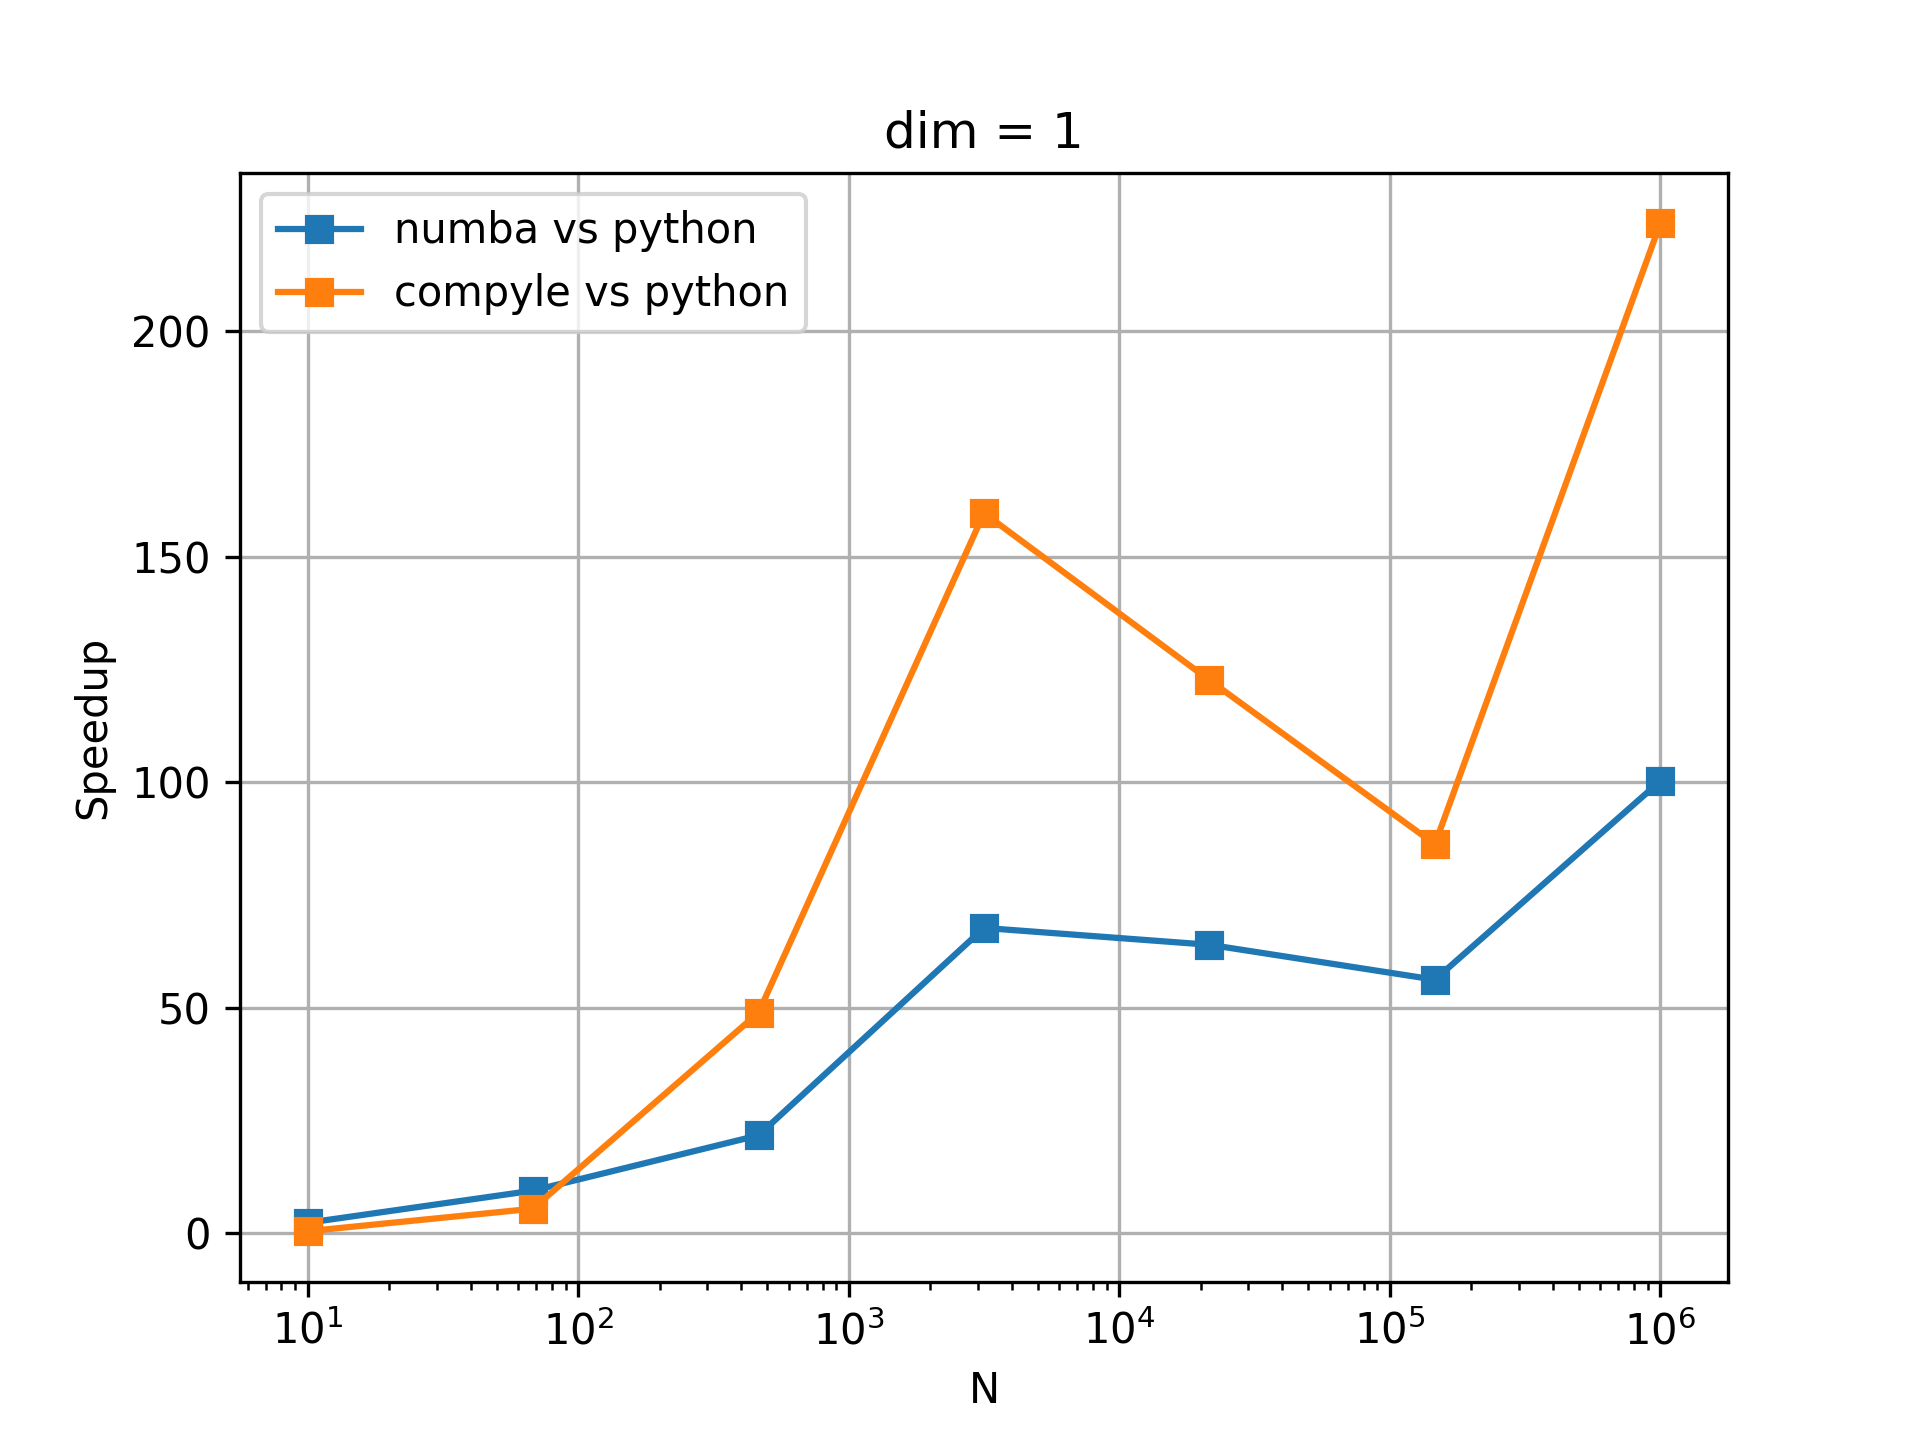
\includegraphics[width=0.8\linewidth]{Code-Figures/espec_speedup_dim_1.png}
	\caption{Speedup of the $1D$ energy spectrum computation for a $1D$ velocity field.}
	\label{fig:espec-dim-1}
\end{figure}
\begin{figure}[h]
    \centering
    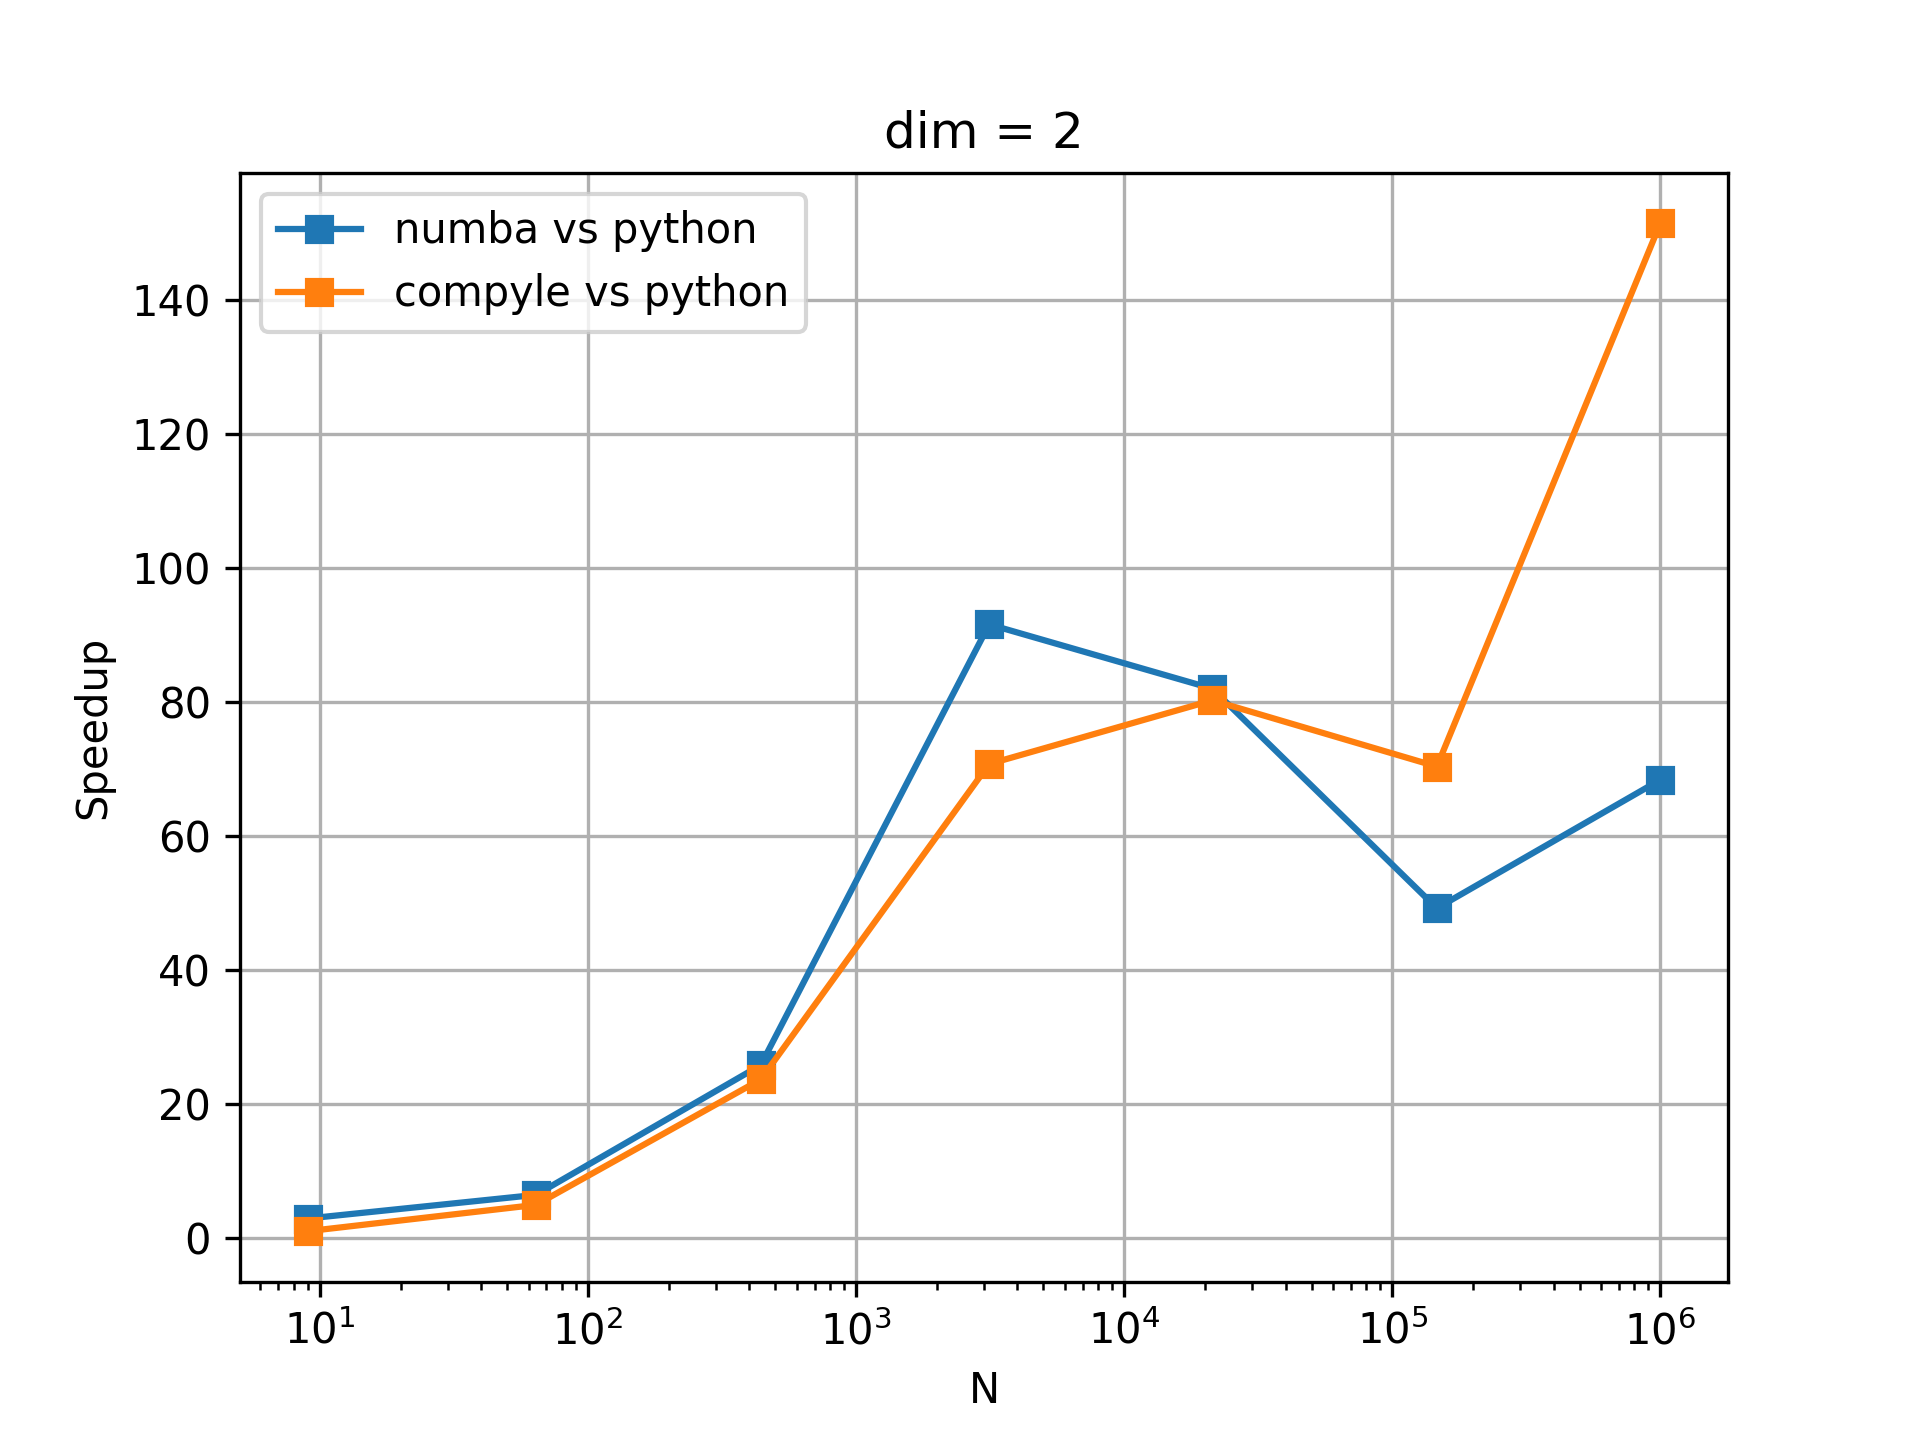
\includegraphics[width=0.8\linewidth]{Code-Figures/espec_speedup_dim_2.png}
    \caption{Speedup of the $1D$ energy spectrum computation for a $2D$ velocity field.}
    \label{fig:espec-dim-2}
\end{figure}
\begin{figure}[h]
    \centering
    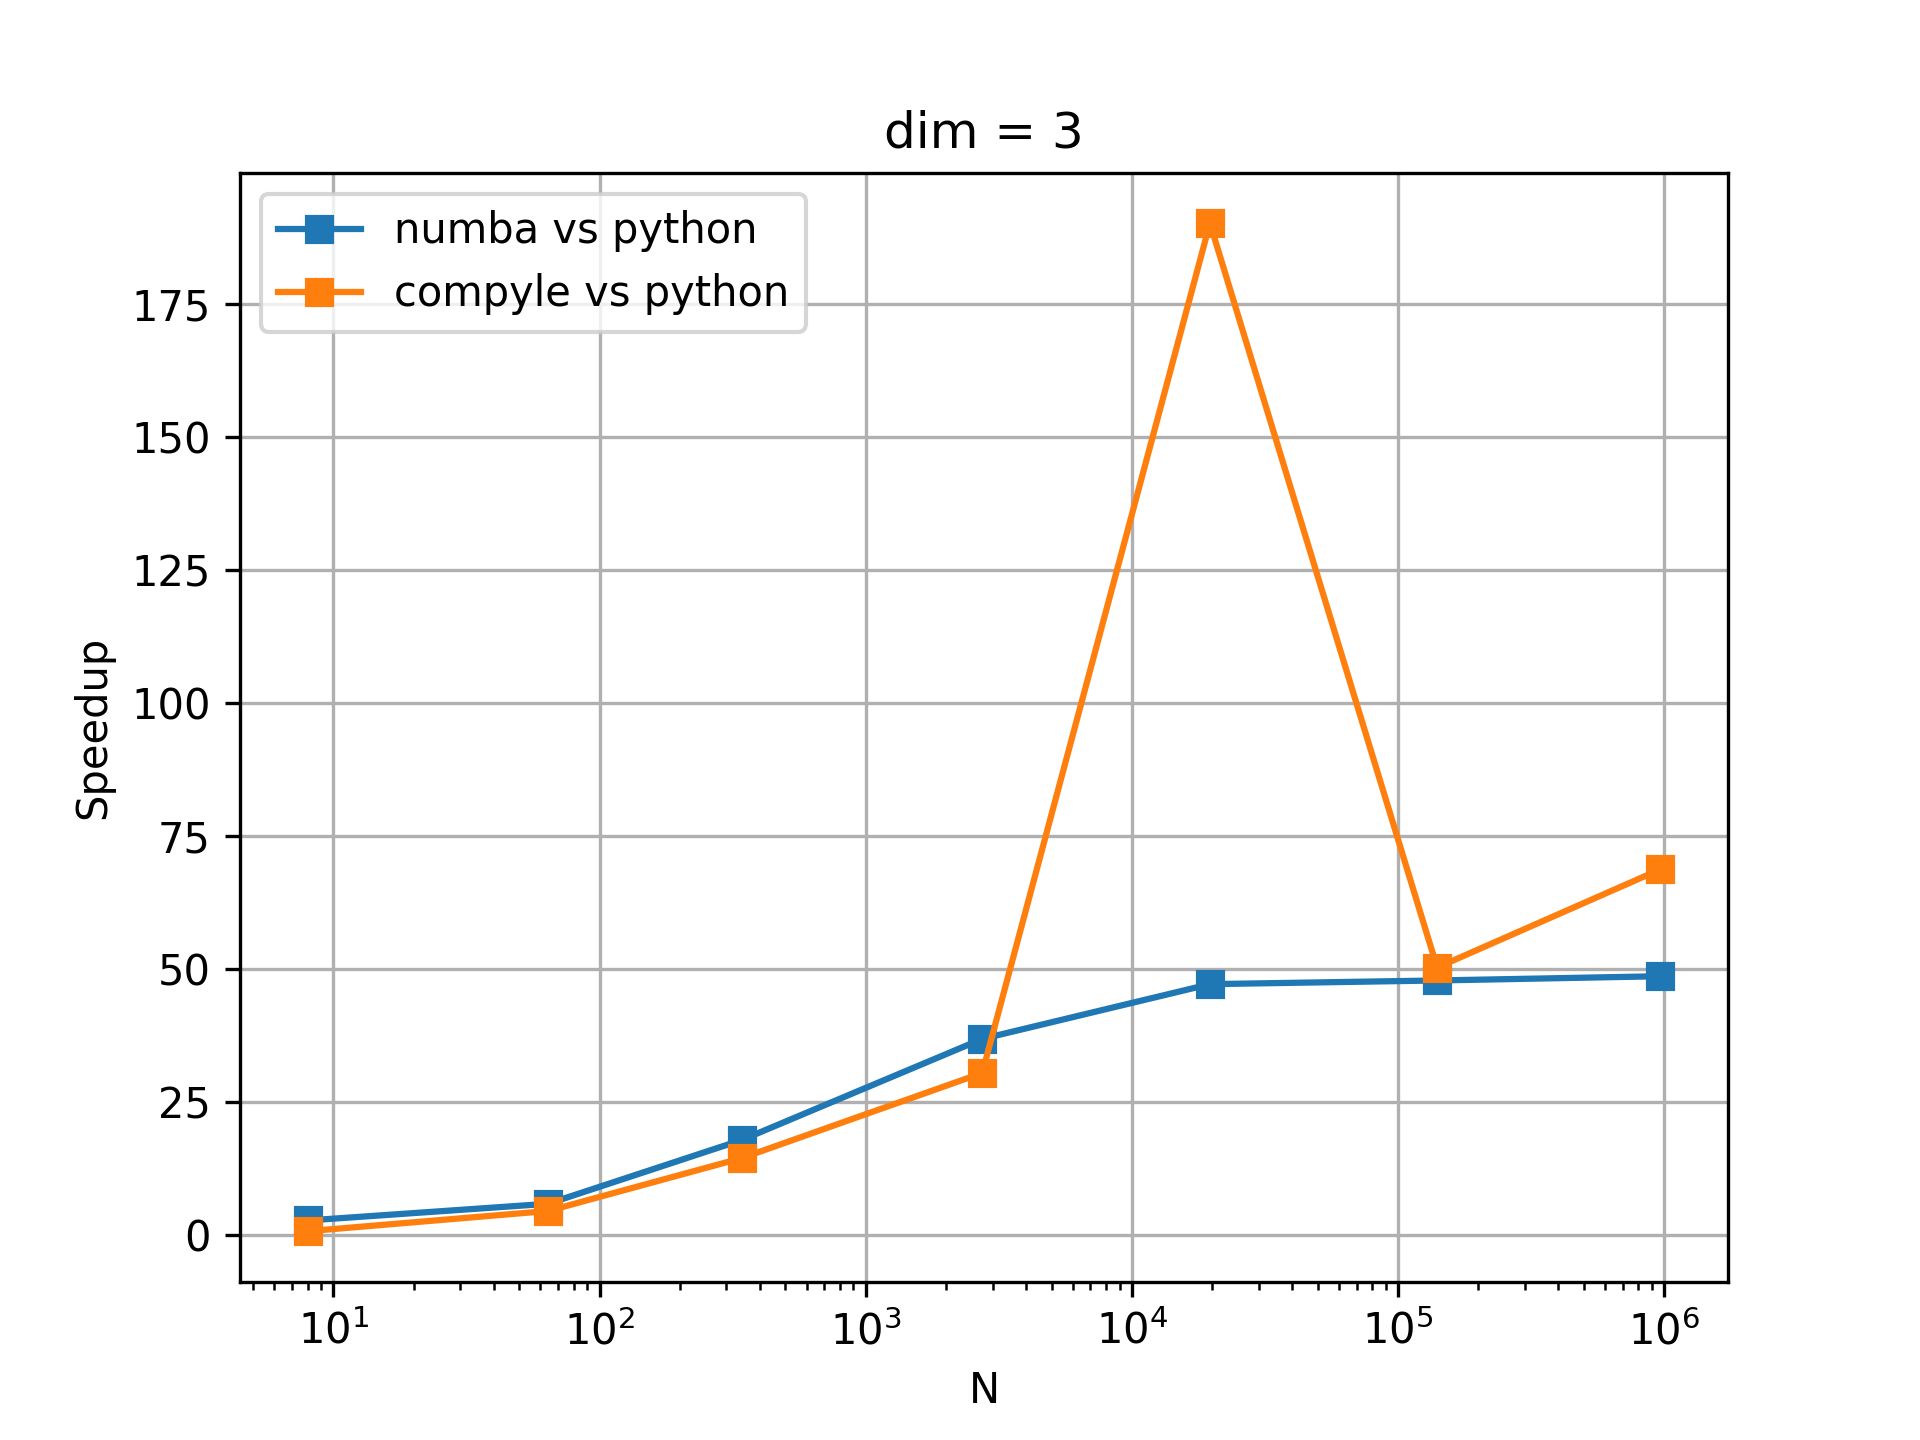
\includegraphics[width=0.8\linewidth]{Code-Figures/espec_speedup_dim_3.png}
    \caption{Speedup of the $1D$ energy spectrum computation for a $3D$ velocity field.}
    \label{fig:espec-dim-3}
\end{figure}

As clearly seen, in the speedup plots, the \texttt{numba} implementation is around $50-100x$ faster than the pure \texttt{python} implementation, while the \texttt{compyle} implementation is around $80-150x$ faster than the pure \texttt{python} implementation over various resolution scales. These trends are observed for all the three dimensions of the velocity field. The \texttt{compyle} implementation, in addition to begin faster than the \texttt{numba} implementation, also has the added advantage of not requiring any additional dependencies, which are not already required by \texttt{PySPH}, unlike the \texttt{numba} implementation, which requires the \texttt{numba} package to be installed separately. Hence, the \texttt{compyle} implementation was chosen for the final implementation of the $1D$ energy spectrum computation.